\chapter{GitHub Enterprise and GitHub Cloud}

\section{About GitHub}

The GitHub integration supports self-hosted GitHub Enterprise or GitHub Cloud.  The integration configurations
are virtually the same for each GitHub platform.  Minor differences may exist due to license or subscription
limitations of your GitHub platform type.  

The GitHub integration, as with other SCM integrations, uses web hooks to emit events to the \cxoneflow endpoint.
GitHub has both organization-level and repository-level webhook configurations
that can be used for simple integration scenarios.  \cxoneflow can also be configured as a GitHub Application
for easier deployment and visibility of deployment.
Deployment as a GitHub Application is the recommended deployment method.


\section{GitHub Application Configuration}

\subsection{Configuring the Application Definition}

The GitHub Application definition determines the owner of the application.  The definition can
be created with an organization as owner or a user as owner.  The configuration method is the same
for each type of ownership.  Deploying with a user as application owner may be disruptive if the user
account is deleted or suspended.

\noindent\\Once the type of ownership is decided, the GitHub Application configuration page can be found in the following
locations:

\begin{itemize}
    \item \textbf{Organization Ownership:} Organization->Settings>Developer Settings->GitHub Apps
    \item \textbf{User Ownership:} User Icon (Top Right)->Settings->Developer Settings->GitHub Apps
\end{itemize}

\noindent\\The following steps can be followed to configure the \cxoneflow GitHub App:

\begin{enumerate}
    \item To start the configuration, click the button "New GitHub App". Figure \ref{fig:gh-new-app} shows
    the GitHub App page with the button to start the configuration in GitHub Enterprise.
    \item Provide a name for the GitHub App as depicted in Figure \ref{fig:gh-app-cfg-1}.  Any name
    can be used, but \cxoneflow is suggested.
    \item Optionally provide a description that is displayed to the users.
    \item Provide a URL that can be used to find information about the \cxoneflow GitHub App.  Any URL
    can be used; the URL to the \cxoneflow GitHub page \textbf{https://github.com/checkmarx-ts/cxone-flow}
    is suggested.
    \item Scroll to the \textbf{Webhook} configuration section; the settings prior to the web hook configuration
    are optional and not used by \cxoneflow.
    \item Provide the URL to the \cxoneflow endpoint with the \textbf{/gh} suffix as shown in Figure \ref{fig:gh-app-cfg-2}.
    \item Provide the web hook secret value that is configured in the \cxoneflow YAML as described in Section \ref{sec:connection-element}.
    \item Scroll the the \textbf{Permissions} section and expand the \textbf{Repository Permissions} as shown in
    Figure \ref{fig:gh-app-cfg-3}.  The following permissions are required:
    \begin{itemize}
        \item Contents: Read-only
        \item Pull requests: Read and write
    \end{itemize}
    \item Scroll to the \textbf{Subscribe to events} section as shown in Figure \ref{fig:gh-app-cfg-4}.  The following events are required:
    \begin{itemize}
        \item Pull request
        \item Pull request review
        \item Push
    \end{itemize}
    \item Scroll to the \textbf{Where can this GitHub App be installed?} section and select \textbf{Any account} as shown in
    Figure \ref{fig:gh-app-cfg-5}.
    \item Click the \textbf{Create GitHub App} button.
    \item After the application is created, open the application settings \textbf{General} tab and scroll to the
    \textbf{Private keys} section as shown in Figure \ref{fig:gh-app-cfg-6}.
    \item Click the \textbf{Generate a private key} button.  A private key entry will appear and a file download will start.
    The contents of the download file is the PEM encoded private key that is to be stored as a secret.  See Section
    \ref{sec:api-auth-element} for configuration instructions to reference this GitHub App private key.
\end{enumerate}

\begin{figure}[ht]
    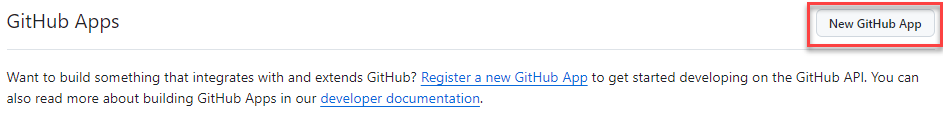
\includegraphics[width=\textwidth]{graphics/gh-new-app.png}
    \caption{New GitHub App Button}
    \label{fig:gh-new-app}
\end{figure}


\begin{figure}[ht]
    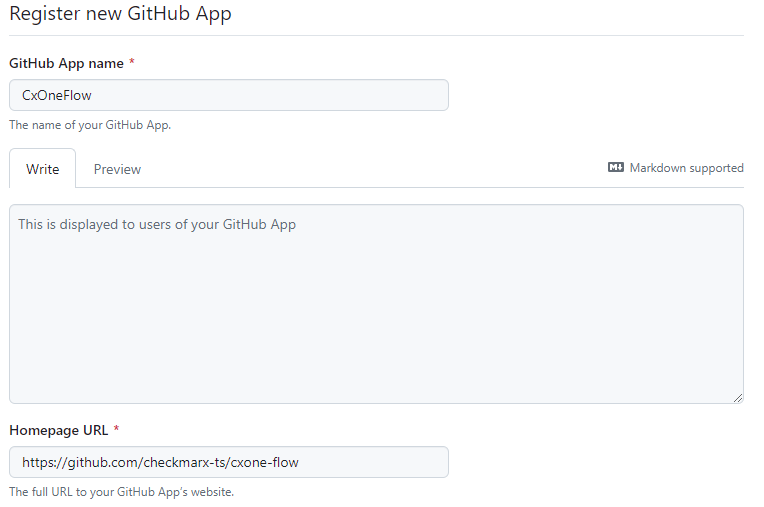
\includegraphics[width=\textwidth]{graphics/gh-app-cfg-1.png}
    \caption{GitHub App Name and URL Configuration}
    \label{fig:gh-app-cfg-1}
\end{figure}

\begin{figure}[ht]
    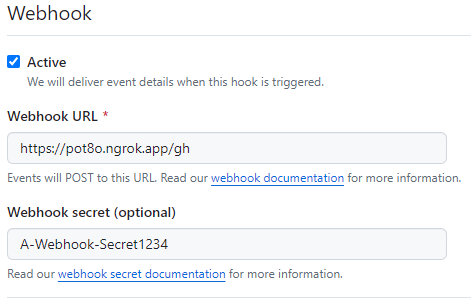
\includegraphics[width=\textwidth]{graphics/gh-app-cfg-2.png}
    \caption{GitHub App Webhook Configuration}
    \label{fig:gh-app-cfg-2}
\end{figure}

\begin{figure}[ht]
    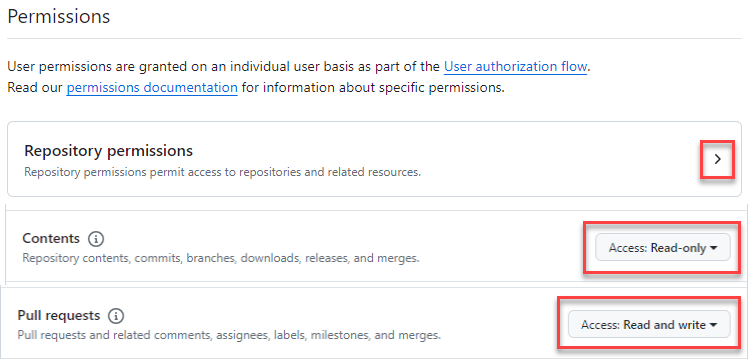
\includegraphics[width=\textwidth]{graphics/gh-app-cfg-3.png}
    \caption{GitHub App Permissions}
    \label{fig:gh-app-cfg-3}
\end{figure}

\begin{figure}[ht]
    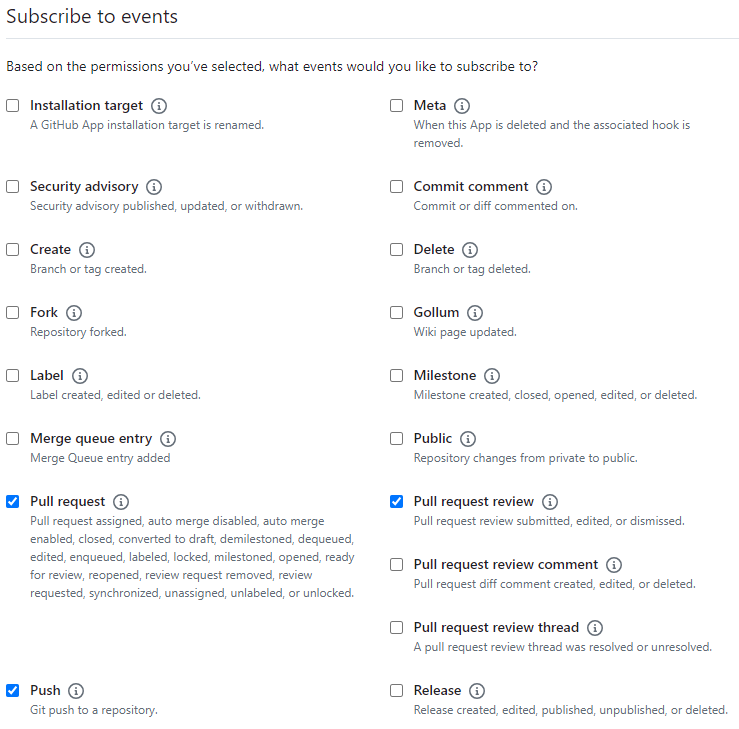
\includegraphics[width=\textwidth]{graphics/gh-app-cfg-4.png}
    \caption{GitHub App Event Subscriptions}
    \label{fig:gh-app-cfg-4}
\end{figure}

\begin{figure}[ht]
    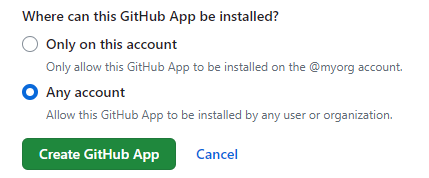
\includegraphics[width=\textwidth]{graphics/gh-app-cfg-5.png}
    \caption{GitHub App Install Scope}
    \label{fig:gh-app-cfg-5}
\end{figure}

\begin{figure}[ht]
    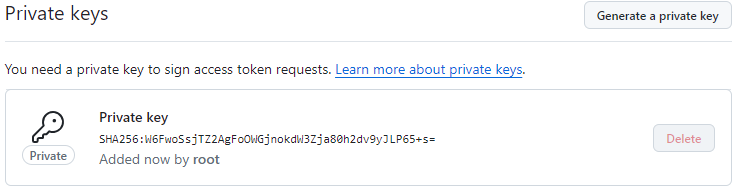
\includegraphics[width=\textwidth]{graphics/gh-app-cfg-6.png}
    \caption{GitHub App Private Keys}
    \label{fig:gh-app-cfg-6}
\end{figure}

\subsection{Deploying the Application}


\section{Webhook Configuration}


\section{Protected Branches}

GitHub allows a default branch to be defined for each repository.  A default branch name is defined at the organization
level and is initially inherited by each repository in the organization.  The default branch may be changed in the repository
to any branch. If there are no branch protection rules for the repository generating a webhook event, the default branch for
the repository is assumed to be a protected branch.

Branch protection rules can be defined at both the organization and repository levels.  If there are any branches
defined as protected via the branch protection rules, those branches are considered protected branches.  When branch protection
rules define protected branches, the repository default branch is not considered as a protected branch.
